\documentclass{hwset}

\name{Erich L Foster}
\class{Calculus I}
\date{29 March 2011}
\assignment{Homework 9}

\begin{document}
\begin{problem}[1.]
	Air is pumped into a spherical balloon at a rate of $20\text{ cm}^3$ per minute. How
	fast is the radius of the balloon increasing when the diameter is $10$ cm?
\end{problem}

\begin{solution}
	\begin{center}
	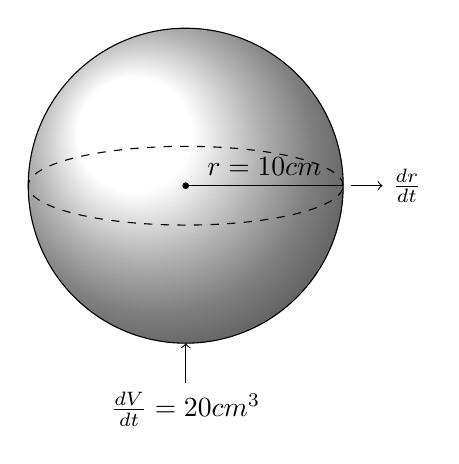
\begin{tikzpicture}
		\filldraw[ball color=white] (0,0) circle (2cm);
		\draw[dashed] (0,0) ellipse(2 and 0.5);
		\draw (0,0) -- (1,0) node[above,fill=none] {$r = 10 \text{ cm}$} -- (2,0);
		\draw[->] (2.1,0) -- (2.5,0) node[right,fill=none] {$\frac{dr}{dt}$};
		\draw[<-] (0,-2) -- (0,-2.5) node[below, fill=none] {$\frac{dV}{dt}=20 \text{ cm}^3$};
		\filldraw[black] (0,0) circle(1pt);
	\end{tikzpicture}
	\end{center}
	The volume of a sphere is
	\begin{align*}
		V& \frac{4}{3} \pi r^3 \\
		\frac{d}{dt}\left[ V \right]&= \frac{d}{dt}\left[ \frac{4}{3} \pi r^3
			\right] \\
		\frac{dV}{dt}&= 4\pi r^2 \frac{dr}{dt} \\
		\frac{dr}{dt}&= \frac{1}{4\pi r^2} \frac{dV}{dt} \\
		\frac{dr}{dt}&= \frac{1}{4\pi 5^2} 20 \\
		\frac{dr}{dt}&= \boxed{\frac{1}{5\pi} \sfrac{\text{cm}}{\text{min}}}.
	\end{align*}
\end{solution}

\begin{problem}[2.]
	A 10-foot ladder is resting against a wall. The bottom of the ladder is
	initially 3 feet away from the wall, and is being pulled away from the wall at
	a rate of $\sfrac{1}{3}$ feet per second. How fast is the top of the ladder
	moving after 4 seconds?
\end{problem}

\begin{solution}
	\begin{center}
	\begin{tikzpicture}
		\draw (0,0) -- (5,0) -- (5,4.7);
		\draw[ultra thick] (3.5,0) -- (5,4.7);
		\draw[|<->|] (3.3,0.2) -- (4.7,4.6);
		\draw[|<->|] (3.5,-0.2) -- (5,-0.2);
		\node at (3.8,2.2) [fill=white, rotate=71] {$z=10\text{ ft}$}; 
		\node at (4.25,-0.6) [fill=white] {$x_0=3\text{ ft}$}; 
		\draw[->] (5.5, 4.7) -- (5.5, 3.8) node[below, fill=white] {$\frac{dy}{dt}$};
		\draw[->] (3.2, 0.2) -- (2.6, 0.2) node[above left, fill=white] {$\frac{dx}{dt} = \frac{1}{3} \sfrac{\text{ft}}{\text{s}}$};
	\end{tikzpicture}
	\end{center}
	The base of the ladder is initially $3$ ft from the wall, however we want to
	know the rate of change in the top of the ladder after $t=4$ s. Therefore, we
	must find the distance the base of the ladder is when $t=4$ s. So,
	\begin{align*}
		x &= x_0 + t\cdot \frac{dx}{dt} \\
		&= 3 + 4\frac{1}{3} \\
		&= \frac{13}{3} \text{ ft}
	\end{align*}
	and 
	\begin{align*}
		y &= \sqrt{z^2 - x^2}\\
		&= \sqrt{10^2 - \left(\frac{13}{3}\right)^2}\\
		&\approx 9.01 \text{ ft}\\
	\end{align*}
	\begin{align*}
		x^2 + y^2 &= z^2\\
		\frac{d}{dt}\left[ x^2 + y^2 \right]&= \frac{d}{dt}\left[ z^2 \right]\\
		2 x\cdot \frac{dx}{dt} + 2 y\cdot \frac{dy}{dt}&= 2 z \cdot
			\cancelto{0}{\frac{dz}{dt}} \\
		\frac{dy}{dt}&= -\dfrac{x \frac{dx}{dt}}{y} \\
		\frac{d3}{dt}&= -\dfrac{\sfrac{4}{3} \cdot \sfrac{1}{3}}{9.01} \\
		\frac{d3}{dt}&\approx \boxed{-0.160 \sfrac{\text{ft}}{\text{s}}}.
	\end{align*}
\end{solution}

\begin{problem}[3.]
	Boat A is traveling east at 30 knots. Boat B is traveling south at 40 knots.
	Suppose the boats are both headed to the same point. How fast is their
	distance from each other decreasing when boat A is 5 nautical miles from its
	destination and boat B is 12 nautical miles from its destination?
\end{problem}

\begin{solution}
	\begin{center}
	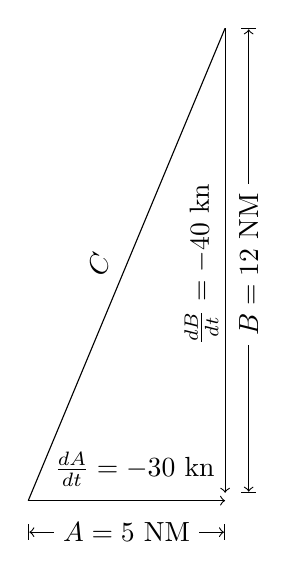
\begin{tikzpicture}
		\draw[->] (0,0) -- (2.5,0);
		\draw[|<->|] (0,-0.4) -- (2.5,-0.4);
		\draw[->] (2.5,6) -- (2.5,0.1);
		\draw[|<->|] (2.8,6) -- (2.8,0.1);
		\draw (0,0) -- (2.5,6);
		\node at (1.25,-0.4) [fill=white] {$A = 5$ NM};
		\node at (1.35,0.4) {$\frac{dA}{dt} = -30$ kn};
		\node at (2.8, 3) [fill=white, rotate=90] {$B = 12$ NM};
		\node at (2.2, 3) [rotate=90] {$\frac{dB}{dt} = -40$ kn};
		\node at (0.9, 3) [fill=white, rotate=72] {$C$};
	\end{tikzpicture}
	\end{center}
	\begin{align*}
		A^2 + B^2 &= C^2 \\
		2A \frac{dA}{dt} + 2B \frac{dB}{dt} &= 2C \frac{dC}{dt} \\
		\frac{dC}{dt} &= \frac{A \frac{dA}{dt} + B \frac{dB}{dt}}{C} \\
		\frac{dC}{dt} &= \frac{A \frac{dA}{dt} + B
			\frac{dB}{dt}}{\sqrt{A^2 + B^2}} \\
		\frac{dC}{dt} &= \frac{-30 \cdot 5 + -40 \cdot 12}{\sqrt{25 + 144}} \\
		\frac{dC}{dt} &= -\frac{630}{13} \\
		\frac{dC}{dt} &\approx \boxed{-48.5 \text{ kn}}.
	\end{align*}
\end{solution}

\begin{problem}[4.]
	Suppose you are sitting on the ground watching a plane flying towards you. The
	plane is flying level at 5000 ft and is traveling 600 mph. If $\theta$ is the
	angle between the ground and your line of sight to the plane, at what rate is
	this angle changing the instant the plane is 5000 ft from you along the
	ground.
\end{problem}

\begin{solution}
	\begin{center}
	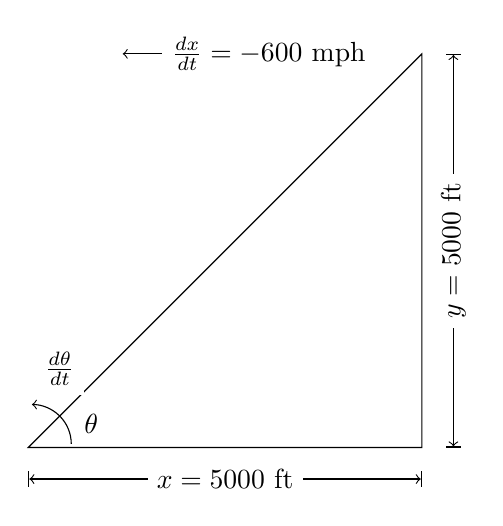
\begin{tikzpicture}
		\draw (0,0) -- (5,0) -- (5,5) -- cycle;
		\draw[|<->|] (0,-0.4) -- (5,-0.4);
		\draw[|<->|] (5.4,0) -- (5.4,5);
		\draw[<-] (1.2,5) -- (1.7,5) node[right] {$\frac{dx}{dt} = -600$ mph};
		\node at (5.4,2.5) [fill=white,rotate=90] {$y=5000$ ft};
		\node at (2.5,-0.4) [fill=white] {$x=5000$ ft};
		\draw[->] (0.4, 0.4) arc(45:90:0.5);
		\draw (0.4, 0.4) arc(45:0:0.5);
		\node at (0.4,1) [fill=white] {$\frac{d\theta}{dt}$};
		\node at (0.8,0.3) [fill=white] {$\theta$};
	\end{tikzpicture}
	\end{center}
	First we must convert $\frac{dL}{dt}$ to ft/sec to have a more reasonable
	answer. Since a change of an angle over an hour really isn't that useful.
	\begin{align*}
		\frac{dL}{dt}&= -600 \sfrac{\text{miles}}{\text{hr}}\\
		&= -600 \sfrac{\text{miles}}{\text{hr}} \cdot 5280
			\sfrac{\text{ft}}{\text{mile}} \cdot \frac{1}{3600}
			\sfrac{\text{hr}}{\text{s}} \\
		&= -880 \sfrac{\text{ft}}{\text{s}}.
	\end{align*}
	Now notice that the angle of inclination is equal to the angle of declination
	and so the equation relating the sides and the angle is
	\begin{align*}
		\tan \theta &= \frac{5000 ft}{x}\\
		\theta &= \tan^{-1} \frac{5000 ft}{x}\\
		\frac{d}{dt}\left[ \theta \right] &= \frac{d}{dt}\left[ \tan^{-1}
			\frac{5000}{x} \right] \\
		\frac{d\theta}{dt} &= -\dfrac{1}{1 + \left(\frac{5000}{x}\right)^2}\cdot
			\frac{5000}{x^2}\cdot \frac{dx}{dt} \\
		\frac{d\theta}{dt} &= \frac{1}{2}\cdot \frac{1}{5000}\cdot 880 \\
		&= \boxed{ 0.088 \sfrac{\text{rad}}{\text{s}}}.
	\end{align*}
\end{solution}

\end{document}
